\NeedsTeXFormat{LaTeX2e}
%
%\documentclass[aps,pra,showpacs,amsmath,amssymb,superscriptaddress,nofootinbib]{revtex4}
\documentclass[]{article}
\usepackage{graphicx}% Include figure files
\usepackage{bm}% bold math
\usepackage{amssymb}
\usepackage{amsmath}
\usepackage{latexsym}
\usepackage{color}
\usepackage{soul}
\usepackage{nopageno}
%%

\begin{document}  

\thispagestyle{empty}

%%%%%%%%%%%%%%%%%%%%%%%%%%%%%%%%  put here figure %%%%%%%%%%%%%%%%%%%%%%%%%%%%%%%%%%%%%%%%%%%%%%%%

\begin{figure}\label{fig:als}
\flushleft
~~~~~~~~~a$_1$)~~~~~~~~~~~~~~~~~~~~~~~~~~~~~~~~~~~~~~~~~~~~b$_1$) \\
\centering
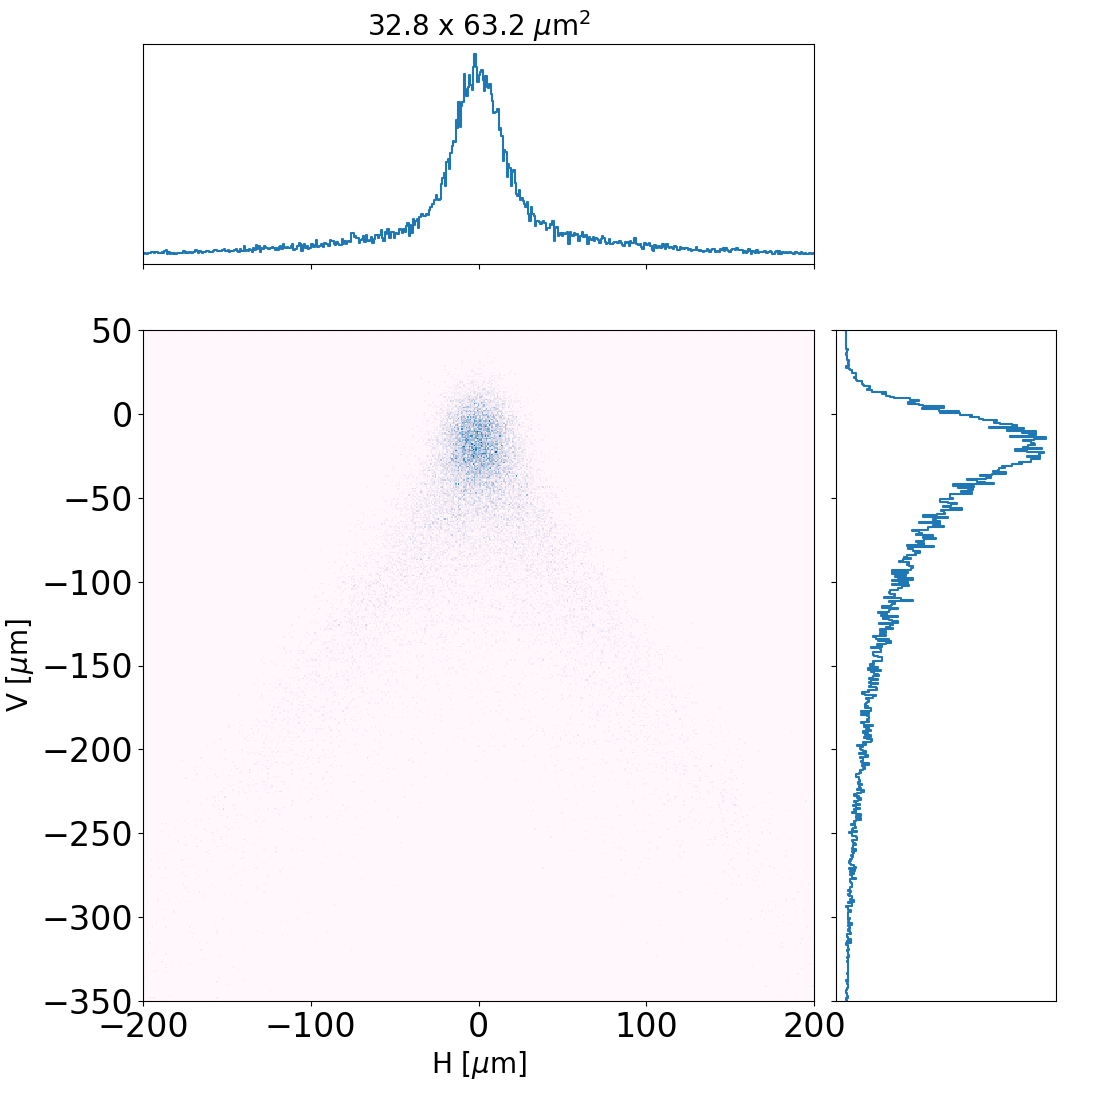
\includegraphics[width=0.45\textwidth]{figures/als_toroid.png}
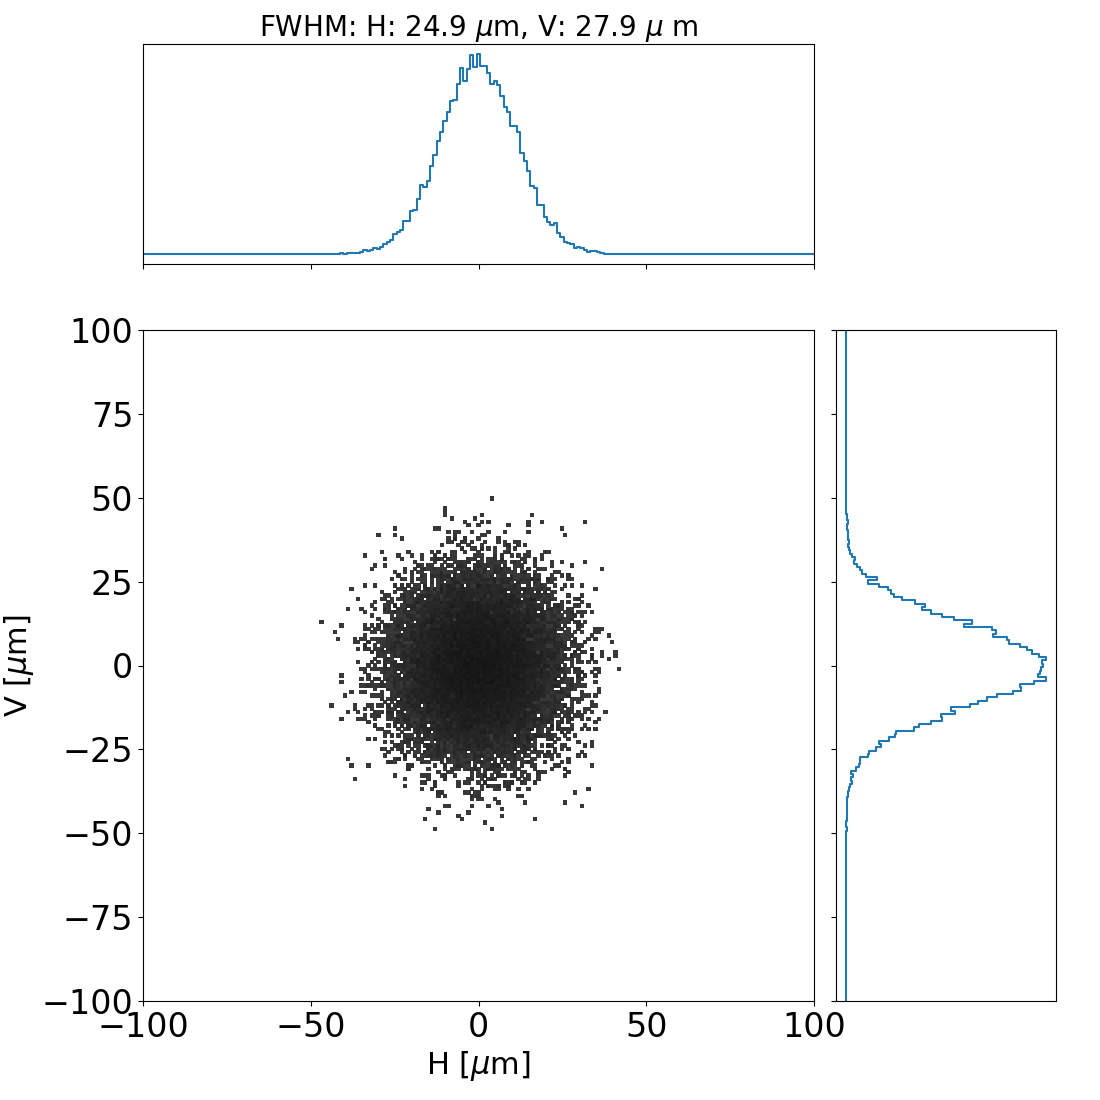
\includegraphics[width=0.45\textwidth]{figures/als_diaboloid.png} \\

\flushleft
~~~~~~~~~a$_2$)~~~~~~~~~~~~~~~~~~~~~~~~~~~~~~~~~~~~~~~~~~~~b$_2$) \\
\centering

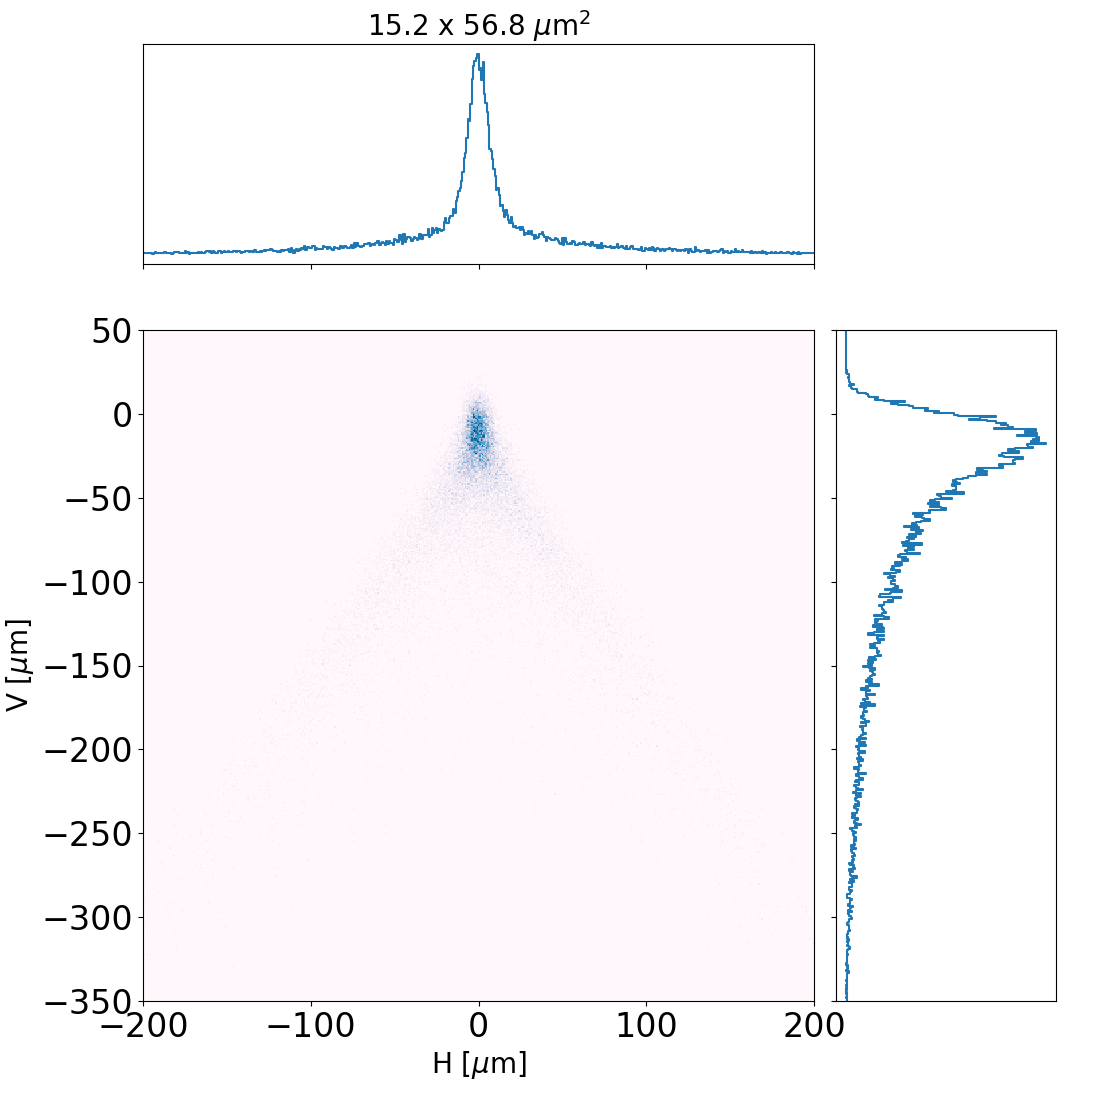
\includegraphics[width=0.45\textwidth]{figures/alsu_toroid.png}
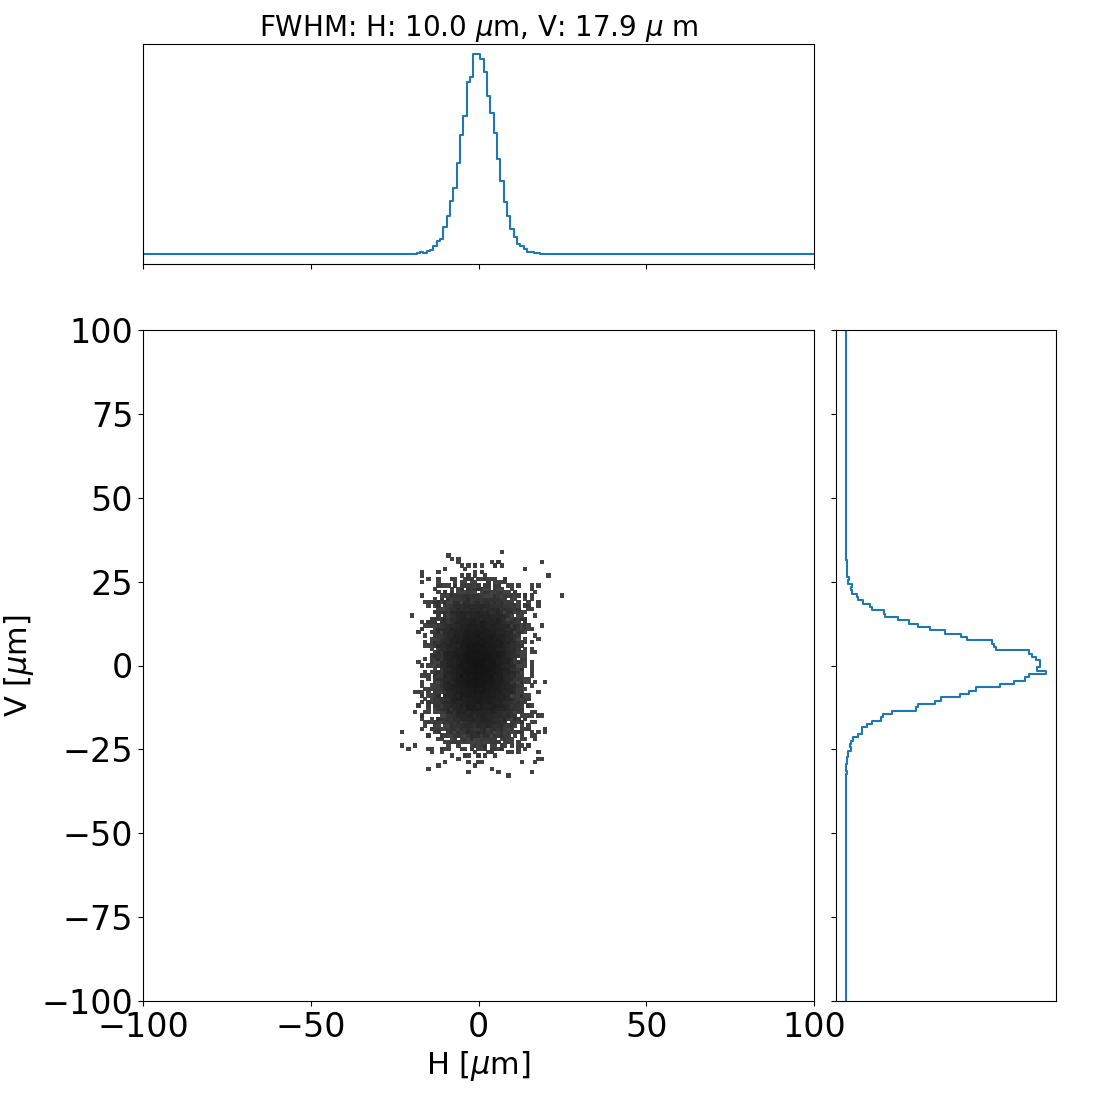
\includegraphics[width=0.45\textwidth]{figures/alsu_diaboloid.png} \\

\flushleft
~~~~~~~~~a$_3$)~~~~~~~~~~~~~~~~~~~~~~~~~~~~~~~~~~~~~~~~~~~~b$_3$) \\
\centering

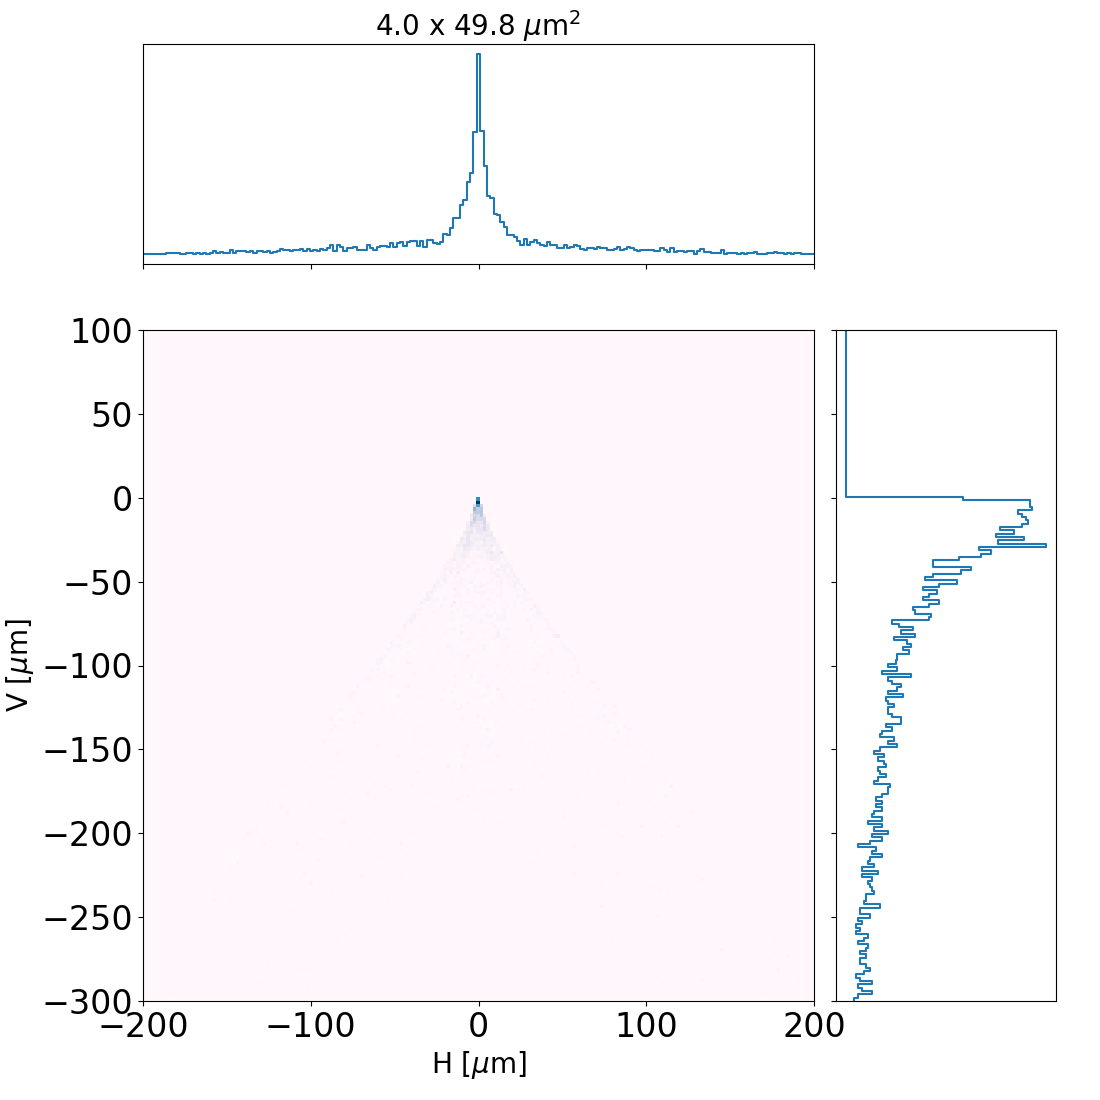
\includegraphics[width=0.45\textwidth]{figures/bl_point_toroid.png} 
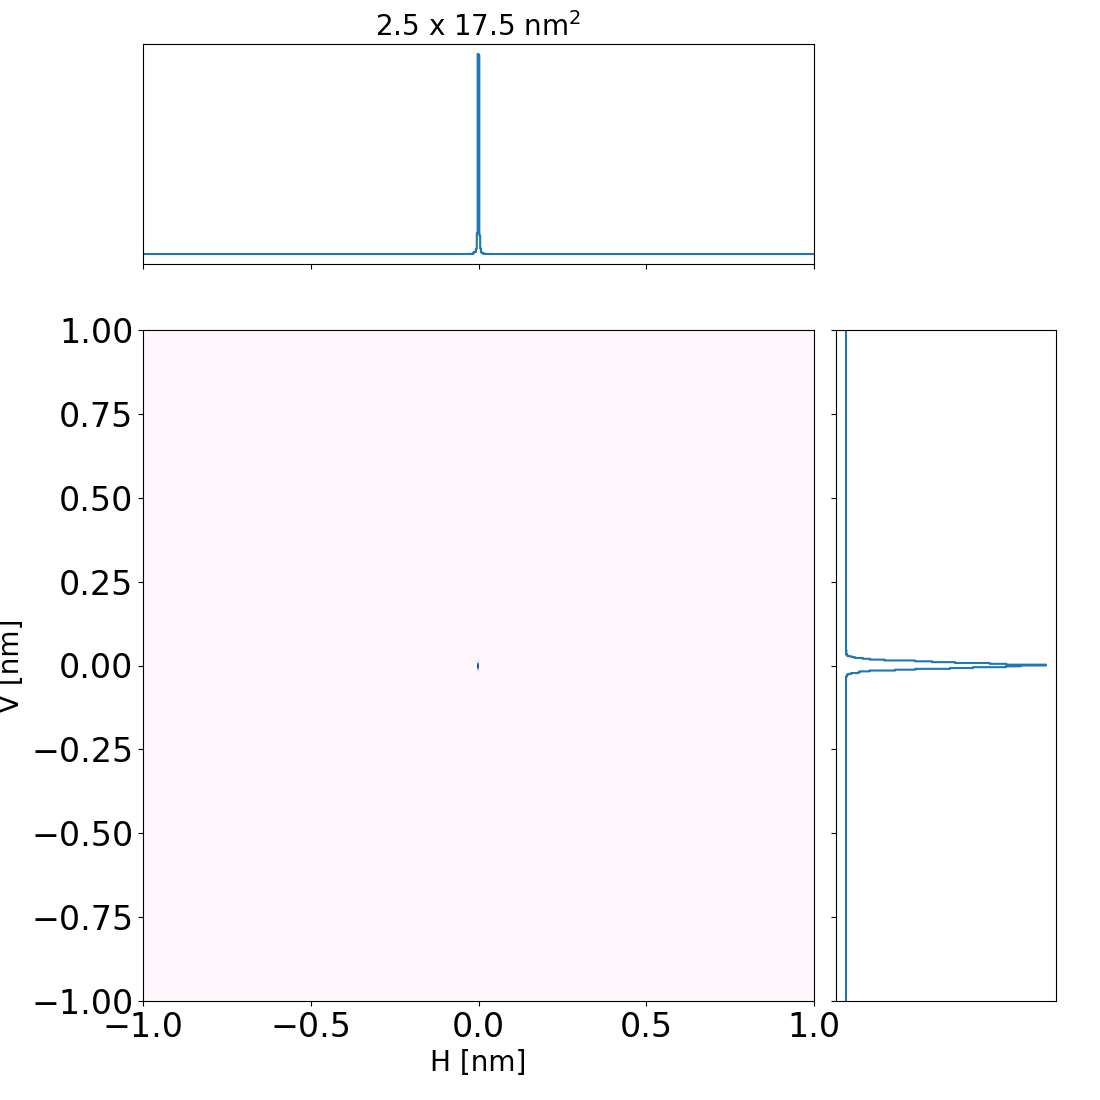
\includegraphics[width=0.45\textwidth]{figures/bl_point_diaboloid-exact.png}  \\
\end{figure}

%%%%%%%%%%%%%%%%%%%%%%%%%%%%%%%%  end put here figure %%%%%%%%%%%%%%%%%%%%%%%%%%%%%%%%%%%%%%%%%%%%%%%%

\end{document}

